\documentclass[sigconf,anonymous,10pt]{acmart}
\settopmatter{printfolios=true}
\makeatletter
\let\@shortauthors\@empty
\makeatother

% Separate supplementary upload; not appended to the technical-content PDF.

\usepackage{longtable}
\usepackage{array}
\usepackage[scaled=0.86]{DejaVuSansMono}
\usepackage{listings}
\lstset{basicstyle=\ttfamily\fontsize{7.4}{8.5}\selectfont,
  columns=fullflexible,keepspaces=true,showstringspaces=false,
  breaklines=true,aboveskip=4pt,belowskip=4pt,
  morekeywords={fn,var,for,in,if,return,let,mod,use,local},
  keywordstyle=\color{blue!65!black},stringstyle=\color{teal!70!black}}

% Keep appendix tables together, without stretch between float blocks.
\makeatletter
\setlength{\@fptop}{0pt}
\setlength{\@fpsep}{10pt}
\setlength{\@fpbot}{0pt plus 1fil}
\makeatother

\setcopyright{none}
\copyrightyear{2027}
\acmYear{2027}
\acmConference[EuroSys '27]{EuroSys 2027}{April 19--23, 2027}{Rabat, Morocco}
\acmISBN{}
\acmDOI{}
\title[Joggle: Malleable Compilation with a Progressive Intermediate Representation]{Joggle: Supplementary Material}

\begin{document}

\onecolumn
\begin{center}
  {\LARGE\bfseries Joggle: Supplementary Material\par}
\end{center}
\vspace{6pt}

\appendix
\renewcommand{\thetable}{A.\arabic{table}}
\setcounter{table}{0}
\section{Operator Measurements}
\label{sec:operator-data}

\begin{table}[h]
  \caption{Operator execution measurements. Joggle revision
  \texttt{5a71fe55a3be}, Apple Clang 17.0.0 (\texttt{-O3 -DNDEBUG}), and
  ONNX Runtime 1.26.0 CPU with one thread and full graph optimization. Each
  entry uses ten warm-ups and 100 measured samples. Ratios divide unrounded
  per-operator medians; values below one indicate lower latency than ORT.
  All 72 subject/variant pairs pass the numerical oracle. The geometric mean
  covers all 24 operators.}
  \label{tab:operator-data}
  \centering
  \small
  \setlength{\tabcolsep}{3pt}
  \begin{tabular}{@{}lrrr@{}}
    \toprule
    Operator & ORT ($\mu$s) & Base / ORT & Opt / ORT \\
    \midrule
    conv-depthwise & 41.92 & 3.64 & 4.57 \\
    conv-pointwise & 63.83 & 146.92 & 32.66 \\
    conv-stem & 178.12 & 4.44 & 9.35 \\
    conv-strided & 39.06 & 171.00 & 190.42 \\
    \midrule
    ew-affine-1k & 2.80 & 0.08 & 0.08 \\
    ew-broadcast-relu & 3.58 & 0.81 & 0.79 \\
    ew-chain-64k & 21.55 & 3.40 & 3.92 \\
    ew-select-16k & 8.08 & 0.98 & 0.87 \\
    \midrule
    fuse-add-relu & 14.11 & 4.89 & 4.53 \\
    fuse-conv-bias-relu & 294.42 & 101.45 & 43.96 \\
    fuse-matmul-bias-relu & 14.26 & 170.18 & 13.35 \\
    fuse-mul-add & 20.34 & 2.32 & 2.44 \\
    \midrule
    mm-batched & 10.64 & 71.02 & 71.00 \\
    mm-rectangular & 13.23 & 214.80 & 9.91 \\
    mm-square-256 & 31.51 & 327.35 & 25.37 \\
    mm-square-64 & 4.55 & 20.57 & 1.66 \\
    \midrule
    quant-conv & 26.51 & 9.06 & 10.25 \\
    quant-dynamic & 4.82 & 1.48 & 1.52 \\
    quant-matmul & 6.15 & 20.78 & 2.40 \\
    quant-qdq-tensor & 3.40 & 0.54 & 0.56 \\
    \midrule
    red-l2-last & 15.46 & 1.10 & 1.07 \\
    red-max-channel & 59.16 & 10.66 & 10.40 \\
    red-mean-spatial & 12.25 & 9.54 & 9.57 \\
    red-sum-row & 9.49 & 5.78 & 6.28 \\
    \midrule
    Geometric mean ratio & --- & 9.27 & 5.21 \\
    Correct operators & 24/24 & 24/24 & 24/24 \\
    \bottomrule
  \end{tabular}
\end{table}

\clearpage
\section{Model Measurements}
\label{sec:model-data}

\begin{table}[!htbp]
  \caption{Model execution latency in milliseconds: median (p50) and p95 of
  100 samples after ten warm-ups. $\times$ denotes an invalid executable.
  Systems use identical input tensors; Table~\ref{tab:model-failures} identifies
  the terminal phase for excluded cases.}
  \label{tab:model-data}
  \centering
  \scriptsize
  \setlength{\tabcolsep}{2.5pt}
  \renewcommand{\arraystretch}{1.18}
  \begin{tabular*}{\textwidth}{@{\extracolsep{\fill}}lrrrrrrrr@{}}
    \toprule
    & \multicolumn{2}{c}{ORT} & \multicolumn{2}{c}{Joggle}
    & \multicolumn{2}{c}{TVM} & \multicolumn{2}{c}{ONNX-MLIR} \\
    \cmidrule(lr){2-3}\cmidrule(lr){4-5}\cmidrule(lr){6-7}\cmidrule(l){8-9}
    Model & p50 & p95 & p50 & p95 & p50 & p95 & p50 & p95 \\
    \midrule
    DenseNet-121 & 18.124 & 20.897 & 706.663 & 715.691 & 1801.893 & 1826.480 & 774.156 & 776.251 \\
    EfficientNet-Lite4 int8 & 11.651 & 13.834 & 131.990 & 133.215 & $\times$ & $\times$ & $\times$ & $\times$ \\
    EfficientNet-Lite4 QDQ & $\times$ & $\times$ & 133.687 & 136.742 & 707.443 & 718.765 & $\times$ & $\times$ \\
    GoogLeNet & 12.390 & 13.356 & 266.846 & 269.242 & 945.052 & 969.546 & 612.744 & 734.218 \\
    MNIST & 0.048 & 0.050 & 0.205 & 0.240 & 0.203 & 0.217 & 0.336 & 0.489 \\
    MobileNetV2 & $\times$ & $\times$ & 86.007 & 86.539 & 181.238 & 182.083 & 23.114 & 23.969 \\
    ResNet-18 & 14.358 & 16.206 & 839.229 & 854.691 & 1129.282 & 1156.727 & 908.751 & 910.927 \\
    ShuffleNet-v2 & 1.858 & 1.936 & 26.912 & 27.141 & 66.672 & 67.064 & 8.450 & 8.667 \\
    SqueezeNet-1.0 QDQ & 2.853 & 3.027 & 56.658 & 57.737 & 164.147 & 165.738 & $\times$ & $\times$ \\
    SqueezeNet-1.1 & 2.263 & 2.437 & 63.121 & 63.634 & 163.041 & 163.570 & 82.522 & 82.958 \\
    SSD-MobileNetV1 & 13.056 & 14.254 & $\times$ & $\times$ & $\times$ & $\times$ & $\times$ & $\times$ \\
    TinyYOLOv3 & 23.817 & 25.145 & 521.532 & 528.014 & $\times$ & $\times$ & 1393.870 & 1410.922 \\
    TinyYOLOv2 & 19.982 & 21.762 & 499.543 & 503.273 & 2421.420 & 2466.986 & 1825.879 & 1955.957 \\
    UltraFace-RFB-320 & 3.414 & 3.778 & 20.767 & 21.067 & $\times$ & $\times$ & 12.112 & 12.845 \\
    XCiT-Tiny & 43.016 & 46.548 & 2953.539 & 2975.516 & 2972.780 & 3007.537 & 318.047 & 321.317 \\
    \midrule
    Correct & \multicolumn{2}{c}{13/15} & \multicolumn{2}{c}{14/15}
    & \multicolumn{2}{c}{11/15} & \multicolumn{2}{c}{11/15} \\
    \bottomrule
  \end{tabular*}
\end{table}

\begin{table}[!htbp]
  \caption{Excluded model executions and the first terminal oracle phase.}
  \label{tab:model-failures}
  \centering
  \scriptsize
  \setlength{\tabcolsep}{4pt}
  \begin{tabular*}{\textwidth}{@{\extracolsep{\fill}}lll@{}}
    \toprule
    System & Backend or preparation failure & Numerical-oracle failure \\
    \midrule
    Joggle & SSD-MobileNetV1 & --- \\
    ORT & --- & EfficientNet-Lite4 QDQ; MobileNetV2 \\
    TVM & EfficientNet-Lite4 int8; SSD-MobileNetV1; TinyYOLOv3; UltraFace & --- \\
    ONNX-MLIR & EfficientNet-Lite4 int8; SqueezeNet-1.0 QDQ; SSD-MobileNetV1 & EfficientNet-Lite4 QDQ \\
    \bottomrule
  \end{tabular*}
\end{table}

\begin{table}[!htbp]
  \caption{Execution controls used for Tables~\ref{tab:operator-data}
  and~\ref{tab:model-data}. Inputs are resident; one execution thread, ten
  warm-ups, and 100 timed samples are used throughout. Joggle times calls in a
  native C loop; the other systems time invocations from the Python collector.
  Numerical checks follow the timed interval.}
  \label{tab:execution-controls}
  \centering
  \scriptsize
  \setlength{\tabcolsep}{5pt}
  \begin{tabular*}{\textwidth}{@{\extracolsep{\fill}}llll@{}}
    \toprule
    System & Optimization & Timed invocation & Output storage \\
    \midrule
    Joggle & Clang 17; \texttt{-O3 -DNDEBUG} & native C harness & caller-allocated buffers \\
    ORT 1.26 & CPU; full graph optimization & \texttt{session.run} & runtime-managed outputs \\
    TVM 0.26.dev0 & default Relax/LLVM; no tuning & \texttt{invoke\_stateful} & VM-managed outputs \\
    ONNX-MLIR 0.4.2 & \texttt{-O3}; no fast math or parallelism & C ABI \texttt{run\_main\_graph} & allocate new; release previous \\
    \bottomrule
  \end{tabular*}
\end{table}

\begin{landscape}
\section{Extension Task Inputs and Outputs}
\label{sec:extension-task-data}

Table~\ref{tab:agent-contracts} records the natural-language contracts and
representative observable inputs and outputs for the 12 tasks used in the
agent and footprint experiments.  Tables~\ref{tab:extension-type}--\ref{tab:extension-layout} specify construction,
verification, and print/parse round trips. Rejected inputs produce no output IR.
Tensor types omit the \texttt{tensor<\ldots{}>} wrapper; bare i8 or f32 denotes a
rank-zero tensor. Axis indices are zero-based.

\scriptsize
\setlength{\tabcolsep}{3pt}
\renewcommand{\arraystretch}{1.12}
\begin{longtable}{@{}p{1.2cm}p{2.5cm}p{6.8cm}p{5.0cm}p{4.5cm}@{}}
\caption{Natural-language task contracts and representative observable inputs
and outputs.  The table preserves the operative semantic constraints while
omitting only system-specific entry-point boilerplate.  Every candidate is
also checked on disjoint hidden cases.}
\label{tab:agent-contracts}\\
\toprule
Family & Task & Natural-language request & Positive input $\rightarrow$ output & Boundary or negative input $\rightarrow$ observation \\
\midrule
\endfirsthead
\multicolumn{5}{l}{\textit{Table~\ref{tab:agent-contracts} continued}}\\
\toprule
Family & Task & Natural-language request & Positive input $\rightarrow$ output & Boundary or negative input $\rightarrow$ observation \\
\midrule
\endhead
\midrule
\multicolumn{5}{r}{\textit{continued on next page}}\\
\endfoot
\bottomrule
\endlastfoot

Definition & \texttt{def-parametric-type} &
Define a signed fixed-point scalar \texttt{fx<W,F>}; require $2\leq W\leq32$
and $0\leq F<W$.  Preserve both parameters through construction, printing,
and reparsing; native function arguments and returns use the new type. &
\texttt{type=fx, W=8, F=3} $\rightarrow$ \texttt{fx<8,3>}, logical width 8 &
\texttt{W=8, F=8} $\rightarrow$ \texttt{invalid-type-parameter} during typing; no output IR \\

Definition & \texttt{def-quantized-op} &
Define \texttt{qadd} on equal-shape i8 tensors.  Input and output scales are
finite and positive; zero points are signed i32.  The result preserves the
operand shape and i8 element type. &
two \texttt{tensor<4xi8>} operands, scales 0.5/0.25/0.5, zeros 0/$-3$/0
$\rightarrow$ \texttt{tensor<4xi8>} &
\texttt{2x3xi8} plus \texttt{3x2xi8} $\rightarrow$ \texttt{shape-mismatch} \\

Analysis & \texttt{ana-broadcast-shape} &
Analyze NumPy trailing-dimension broadcasting for nonnegative extents.  Pad
the shorter shape with leading ones; aligned extents must be equal or one,
and a one selects the other extent, including zero. &
\texttt{[2,3,1]}, \texttt{[4]} $\rightarrow$ legal, \texttt{[2,3,4]} &
\texttt{[2,3]}, \texttt{[4,3]} $\rightarrow$ illegal, conflict axis 1 from the end \\

Analysis & \texttt{ana-numeric-range} &
Propagate closed finite intervals through add, multiply, ReLU, and clamp;
multiplication evaluates all four endpoint products. &
\texttt{mul([-2,3],[-4,5])} $\rightarrow$ \texttt{[-12,15]} &
\texttt{relu([2,-1])} $\rightarrow$ \texttt{invalid-interval} \\

Rewrite & \texttt{rew-add-zero} &
Replace integer add-by-zero when type and shape are preserved.  Floating
positive zero additionally requires \texttt{no\_signed\_zeros}; retain
negative zero.  Remove a matched constant only when it has no remaining uses. &
f32 \texttt{x+0}, shape \texttt{[4]}, \texttt{no\_signed\_zeros=true}
$\rightarrow$ replace by \texttt{x} &
f32 \texttt{x+0.001} $\rightarrow$ keep operation \\

Rewrite & \texttt{rew-redundant-cast} &
Remove identity casts and cancel round trips only for lossless signed-integer
widening or finite f32-to-f64 widening.  Keep narrowing, float--integer, and
shape-changing conversions. &
\texttt{f32[4] -> f32[4]} $\rightarrow$ eliminate cast &
\texttt{i16[4] -> i8[4] -> i16[4]} $\rightarrow$ retain casts \\

Conversion & \texttt{con-gelu-expand} &
Replace native SSA \texttt{gelu} by
$0.5x(1+\operatorname{erf}(x/\sqrt{2}))$ using declared primitive targets.
Preserve shape, floating element type, and every output user. &
\makebox[\linewidth][c]{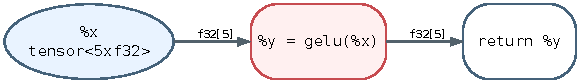
\includegraphics[width=0.92\linewidth]{figures/agent-gelu-before.pdf}}\par
\texttt{gelu}, f32, shape \texttt{[5]} &
\makebox[\linewidth][c]{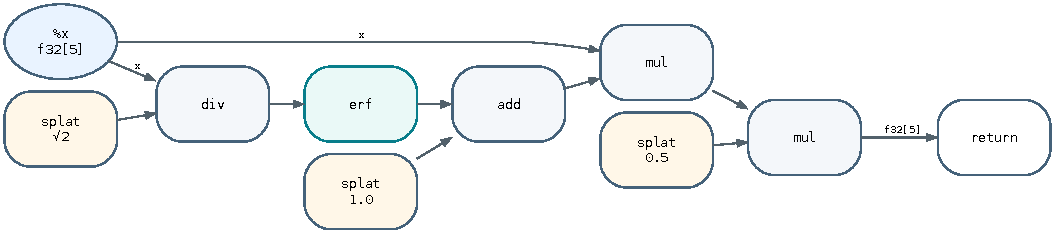
\includegraphics[width=0.92\linewidth]{figures/agent-gelu-after.pdf}}\par
no \texttt{gelu}; graph contains \texttt{erf}. Integer input
$\rightarrow$ \texttt{unsupported-element-type}; no output IR \\

Conversion & \texttt{con-quant-expand} &
Convert i8 tensor \texttt{qadd} into two dequantizations, f32 add, and
quantization with ties-to-even rounding and i8 saturation.  Preserve shape
and result users. &
\texttt{[-3,0,5,120]} plus \texttt{[2,1,-8,120]}, scale 0.5
$\rightarrow$ \texttt{[-1,1,-3,127]} &
negative scale $\rightarrow$ \texttt{invalid-scale}; no output IR \\

Emission & \texttt{emit-graph-manifest} &
Emit deterministic schema-v1 JSON from a typed SSA function.  Number nodes
and values in stable order; preserve repeated operands, output order, types,
and sorted user attributes; omit declarations and source names. &
\texttt{splat -> add -> relu} $\rightarrow$ nodes \texttt{n0..n2}, values
\texttt{v0..v3}, output \texttt{v3} &
Repeated emission $\rightarrow$ byte-identical JSON \\

Emission & \texttt{emit-kernel-wrapper} &
Emit a complete C99 translation unit exporting
\texttt{task\_kernel(input,output,count)} for ReLU or $2x+1$.  Support exact
in-place execution and zero count; do not touch guards or nonaliased inputs. &
ReLU on \texttt{[-2,-0,1.5,4]} $\rightarrow$ \texttt{[+0,+0,1.5,4]} &
\texttt{count=0}, null pointers $\rightarrow$ no access; compiled driver and guard oracle pass \\

Vertical & \texttt{vert-int4} &
Add signed qint4 values, saturate to $[-8,7]$, and pack two's-complement
nibbles low-first.  For odd counts, zero the unused high nibble.  Reject
out-of-range source literals before addition. &
\texttt{[-8,-1,0,3,7]} plus \texttt{[1,1,-2,6,7]}
$\rightarrow$ \texttt{[-7,0,-2,7,7]}, bytes \texttt{09 7e 07} &
literal 8 $\rightarrow$ \texttt{literal-out-of-range} \\

Vertical & \texttt{vert-fused-op} &
Add NHWC/HWIO signed-i8 \texttt{fused\_qconv\_relu}: valid unit-stride
cross-correlation, i32 bias, ties-to-even requantization, i8 saturation, and
real-domain ReLU.  Fuse only a single-use qconv--bias--requantize--ReLU chain. &
unit kernel with input \texttt{[1,-2]}, weights \texttt{[2,-3]}, bias 1
$\rightarrow$ \texttt{[4]} and one fused manifest node &
shared convolution result $\rightarrow$ no match; original chain preserved \\

\end{longtable}
\end{landscape}

\subsection{Parametric Type Definition}
\begin{table}[H]
\caption{\texttt{def-parametric-type}: complete inputs and expected outputs.
Width denotes logical bits, not ABI allocation size.}
\label{tab:extension-type}
\centering
\scriptsize
\setlength{\tabcolsep}{3pt}
\begin{tabular*}{\textwidth}{@{\extracolsep{\fill}}llllll@{}}
\toprule
Case & Width & Fraction bits & Expected type & Logical bits & Expected diagnostic \\
\midrule
fx8-3 & 8 & 3 & \texttt{fx<8,3>} & 8 & --- \\
fx16-7 & 16 & 7 & \texttt{fx<16,7>} & 16 & --- \\
minimum-integer & 2 & 0 & \texttt{fx<2,0>} & 2 & --- \\
minimum-fraction & 2 & 1 & \texttt{fx<2,1>} & 2 & --- \\
maximum-integer & 32 & 0 & \texttt{fx<32,0>} & 32 & --- \\
maximum-fraction & 32 & 31 & \texttt{fx<32,31>} & 32 & --- \\
fraction-overflow & 8 & 8 & --- & --- & invalid-type-parameter \\
width-too-small & 1 & 0 & --- & --- & invalid-type-parameter \\
width-too-large & 33 & 0 & --- & --- & invalid-type-parameter \\
negative-width & -2 & 0 & --- & --- & invalid-type-parameter \\
negative-fraction & 8 & -1 & --- & --- & invalid-type-parameter \\
\bottomrule
\end{tabular*}
\end{table}

\subsection{Quantized Operation Definition}
\begin{table}[H]
\caption{\texttt{def-quantized-op}: complete inputs and expected outputs, with
defaults expanded. Scales are finite positive f64 values; zero points are signed
i32 values. This task defines the operation; arithmetic lowering is evaluated separately.}
\label{tab:extension-qadd}
\centering
\scriptsize
\setlength{\tabcolsep}{3pt}
\begin{tabular*}{\textwidth}{@{\extracolsep{\fill}}llllll@{}}
\toprule
Case & LHS type & RHS type & Scales (L, R, out) & Zero points (L, R, out) & Expected result / diagnostic \\
\midrule
vector & 4$\times$i8 & 4$\times$i8 & 0.5, 0.25, 0.5 & 0, -3, 0 & 4$\times$i8 \\
matrix & 2$\times$3$\times$i8 & 2$\times$3$\times$i8 & 0.125, 0.125, 0.25 & 2, 2, 1 & 2$\times$3$\times$i8 \\
scalar & i8 & i8 & 1, 1, 0.25 & 0, 0, 0 & i8 \\
empty-axis & 0$\times$3$\times$i8 & 0$\times$3$\times$i8 & 1, 1, 0.5 & 0, 0, 0 & 0$\times$3$\times$i8 \\
signed-zero-point-bounds & 1$\times$2$\times$3$\times$i8 & 1$\times$2$\times$3$\times$i8 & 0.0625, 2, 1 & $-$2$^{31}$, 2$^{31}$$-$1, $-$2$^{31}$ & 1$\times$2$\times$3$\times$i8 \\
shape-mismatch & 2$\times$3$\times$i8 & 3$\times$2$\times$i8 & 1, 1, 0.5 & 0, 0, 0 & shape-mismatch \\
zero-scale & 4$\times$i8 & 4$\times$i8 & 1, 1, 0 & 0, 0, 0 & invalid-scale \\
lhs-zero-scale & 4$\times$i8 & 4$\times$i8 & 0, 1, 1 & 0, 0, 0 & invalid-scale \\
rhs-negative-scale & 4$\times$i8 & 4$\times$i8 & 1, -0.25, 1 & 0, 0, 0 & invalid-scale \\
negative-output-scale & 4$\times$i8 & 4$\times$i8 & 1, 1, -0.5 & 0, 0, 0 & invalid-scale \\
lhs-element & 4$\times$i16 & 4$\times$i8 & 1, 1, 1 & 0, 0, 0 & operand-type-mismatch \\
rhs-element & 4$\times$i8 & 4$\times$i16 & 1, 1, 1 & 0, 0, 0 & operand-type-mismatch \\
rank-mismatch & i8 & 1$\times$i8 & 1, 1, 1 & 0, 0, 0 & shape-mismatch \\
\bottomrule
\end{tabular*}
\end{table}

\subsection{Layout-Carrying Operation Definition}
\begin{table}[H]
\caption{\texttt{def-layout-attribute}: complete inputs and expected outputs.
The constructor infers the result shape and preserves the element type and both layout attributes.}
\label{tab:extension-layout}
\centering
\scriptsize
\setlength{\tabcolsep}{3pt}
\begin{tabular*}{\textwidth}{@{\extracolsep{\fill}}llllll@{}}
\toprule
Case & Input type & Source & Destination & Permutation & Expected result / diagnostic \\
\midrule
to-nhwc & 1$\times$3$\times$8$\times$16$\times$f32 & NCHW & NHWC & 0, 2, 3, 1 & 1$\times$8$\times$16$\times$3$\times$f32 \\
to-nchw & 2$\times$7$\times$9$\times$4$\times$f16 & NHWC & NCHW & 0, 3, 1, 2 & 2$\times$4$\times$7$\times$9$\times$f16 \\
identity-nchw & 2$\times$3$\times$4$\times$5$\times$f32 & NCHW & NCHW & 0, 1, 2, 3 & 2$\times$3$\times$4$\times$5$\times$f32 \\
identity-nhwc & 2$\times$4$\times$5$\times$3$\times$f16 & NHWC & NHWC & 0, 1, 2, 3 & 2$\times$4$\times$5$\times$3$\times$f16 \\
empty-axis & 1$\times$3$\times$0$\times$16$\times$f32 & NCHW & NHWC & 0, 2, 3, 1 & 1$\times$0$\times$16$\times$3$\times$f32 \\
integer-element & 1$\times$8$\times$16$\times$3$\times$i8 & NHWC & NCHW & 0, 3, 1, 2 & 1$\times$3$\times$8$\times$16$\times$i8 \\
wrong-rank & 3$\times$8$\times$16$\times$f32 & NCHW & NHWC & --- & rank-mismatch \\
scalar-rank & f32 & NCHW & NHWC & --- & rank-mismatch \\
invalid-source & 1$\times$3$\times$8$\times$16$\times$f32 & CHWN & NHWC & --- & invalid-layout \\
invalid-destination & 1$\times$3$\times$8$\times$16$\times$f32 & NCHW & HWCN & --- & invalid-layout \\
\bottomrule
\end{tabular*}
\end{table}

\clearpage
\subsection{Graph Transformations and Numerical Checks}
\label{sec:graph-cases}

\begin{table}[!htbp]
\centering\scriptsize
\caption{Reference graph transformations and observable outputs for five
extension tasks. Coral marks matched operations, teal the replacement, and
blue typed inputs. Graphs and values show the task contracts' expected results.
RNE denotes round-to-nearest, ties-to-even.}
\label{tab:graph-cases}
\setlength{\tabcolsep}{5pt}
\renewcommand{\arraystretch}{1.15}
\begin{tabular}{@{}>{\centering\arraybackslash}m{\dimexpr0.5\textwidth-5pt\relax}>{\centering\arraybackslash}m{\dimexpr0.5\textwidth-5pt\relax}@{}}
\toprule
Before & After \\
\midrule
\multicolumn{2}{@{}p{\textwidth}@{}}{\textbf{Remove add-by-zero.}\quad\texttt{rew-add-zero}\par
f32[4], positive zero, \texttt{no\_signed\_zeros}. All users now read
\texttt{\%x}; adding 0.001 retains the add.} \\*[2pt]
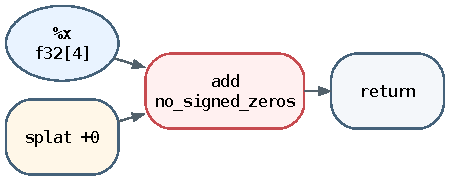
\includegraphics[width=6.4cm,height=1.65cm,keepaspectratio]{figures/task-zero-before.pdf} &
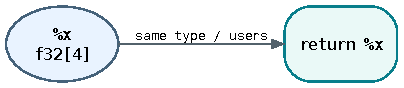
\includegraphics[width=6.4cm,height=1.65cm,keepaspectratio]{figures/task-zero-after.pdf} \\[5pt]
\midrule
\multicolumn{2}{@{}p{\textwidth}@{}}{\textbf{Cancel a lossless cast round trip.}\quad\texttt{rew-redundant-cast}\par
i8$\to$i16$\to$i8 preserves \texttt{[-128,-1,0,127]}.
i16$\to$i8$\to$i16 retains both casts.} \\*[2pt]
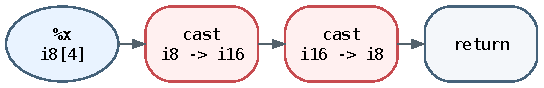
\includegraphics[width=6.4cm,height=1.65cm,keepaspectratio]{figures/task-cast-before.pdf} &
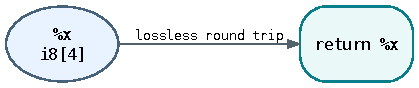
\includegraphics[width=6.4cm,height=1.65cm,keepaspectratio]{figures/task-cast-after.pdf} \\[5pt]
\midrule
\multicolumn{2}{@{}p{\textwidth}@{}}{\textbf{Expand GELU.}\quad\texttt{con-gelu-expand}\par
$y=0.5x(1+\operatorname{erf}(x/\sqrt{2}))$. Preserve f32[5] and every
output user; reject integer inputs.} \\*[2pt]
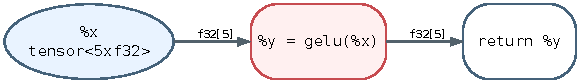
\includegraphics[width=6.4cm,height=1.65cm,keepaspectratio]{figures/agent-gelu-before.pdf} &
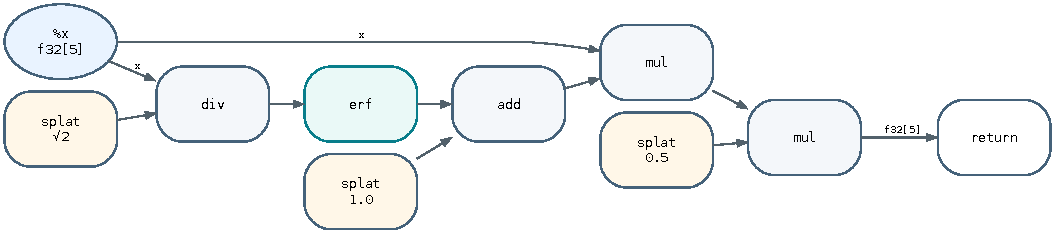
\includegraphics[width=6.4cm,height=1.65cm,keepaspectratio]{figures/agent-gelu-after.pdf} \\[5pt]
\midrule
\multicolumn{2}{@{}p{\textwidth}@{}}{\textbf{Expand quantized addition.}\quad\texttt{con-quant-expand}\par
\texttt{[-3,0,5,120]+[2,1,-8,120]} $\to$ \texttt{[-1,1,-3,127]};
all scales 0.5 and zero points 0. Reject negative scales.} \\*[2pt]
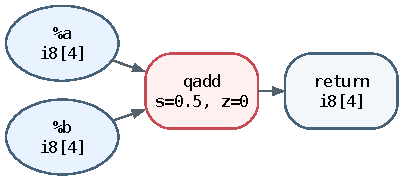
\includegraphics[width=6.4cm,height=1.65cm,keepaspectratio]{figures/task-quant-before.pdf} &
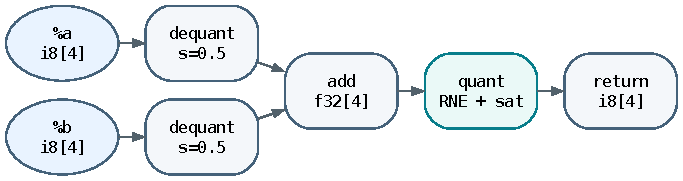
\includegraphics[width=6.4cm,height=1.65cm,keepaspectratio]{figures/task-quant-after.pdf} \\[5pt]
\midrule
\multicolumn{2}{@{}p{\textwidth}@{}}{\textbf{Fuse a single-use quantized chain.}\quad\texttt{vert-fused-op}\par
\texttt{x=[1,-2], w=[2,-3]}, bias 1; accumulator 9, scales 0.25/0.5:
RNE(4.5)$=4$. Shared convolution results retain the original chain.} \\*[2pt]
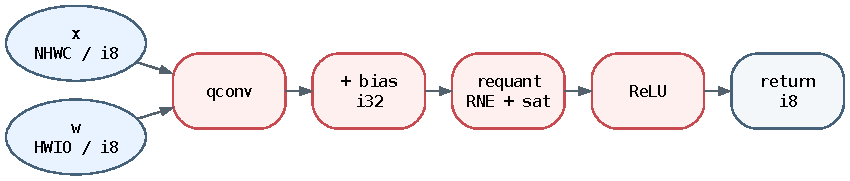
\includegraphics[width=6.4cm,height=1.65cm,keepaspectratio]{figures/task-fusion-before.pdf} &
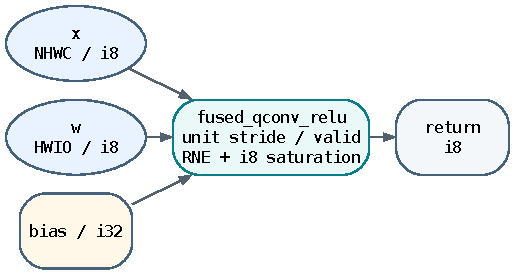
\includegraphics[width=6.4cm,height=1.65cm,keepaspectratio]{figures/task-fusion-after.pdf} \\[5pt]
\bottomrule
\end{tabular}
\end{table}

\begin{table}[!htbp]
\centering\scriptsize
\caption{Worked analysis and artifact-output checks. Values are task-contract
expectations; byte strings are hexadecimal.}
\label{tab:worked-outputs}
\setlength{\tabcolsep}{5pt}
\renewcommand{\arraystretch}{1.2}
\begin{tabular}{@{}p{2.6cm}p{4.2cm}p{4.7cm}p{5.0cm}@{}}
\toprule
Task / case & Input & Intermediate computation & Expected observable output \\
\midrule
Broadcast / empty axis &
\texttt{[2,0]}, \texttt{[1]} &
Align \texttt{[2,0]} with \texttt{[1,1]} &
legal; shape \texttt{[2,0]} \\
Interval / mixed product &
\texttt{[-2,3]} $\times$ \texttt{[-4,5]} &
Endpoint products \texttt{[8,-10,-12,15]} &
interval \texttt{[-12,15]} \\
Interval / add then ReLU &
\texttt{[-3,2] + [1,4]} &
Sum \texttt{[-2,6]}, then clamp below at 0 &
interval \texttt{[0,6]} \\
Manifest / repeated edges &
\texttt{add(arg,arg)};\par return \texttt{[twice,arg,twice]} &
\texttt{arg=v0}, \texttt{twice=v1}, node \texttt{n0} &
inputs \texttt{[v0,v0]};\par outputs \texttt{[v1,v0,v1]} \\
Wrapper / affine &
f32 \texttt{[-2,0,1.5,4]} &
Separate f32 multiply by 2, then add 1 &
\texttt{[-3,1,4,9]}; same result in-place \\
qint4 / odd count &
\texttt{[-8,-1,0,3,7]} $+$ \texttt{[1,1,-2,6,7]} &
i8 sums \texttt{[-7,0,-2,9,14]}; saturate &
\texttt{[-7,0,-2,7,7]}; bytes \texttt{09 7e 07} \\
qint4 / negative tail &
\texttt{[-8] + [-8]} &
Saturate $-16$ to $-8$; zero high nibble &
\texttt{[-8]}; byte \texttt{08} \\
\bottomrule
\end{tabular}
\end{table}

\clearpage
\section{Repeated Model Updates}
\label{sec:update-data}
\begin{table}[!htbp]
\centering\scriptsize
\caption{Ten paired repetitions at each of nine edit sites. Times are seconds; brackets give the interquartile range. Speedup is the median of paired rebuild/update ratios. Each pass count covers ten rebuilds and ten updates.}
\label{tab:update-sites}
\setlength{\tabcolsep}{4pt}
\renewcommand{\arraystretch}{1.12}
\begin{tabular*}{\textwidth}{@{\extracolsep{\fill}}lllrrrc@{}}
\toprule Model & Edit node & System & Rebuild [Q1, Q3] & Update [Q1, Q3] & Speedup & Pass \\
\midrule
DenseNet-121 & 5-add & Joggle & 51.029 [49.521, 51.807] & 20.420 [20.109, 20.568] & $2.49\times$ & 20/20 \\
 &  & TVM & 10.413 [10.334, 10.531] & 10.531 [10.469, 10.628] & $0.99\times$ & 20/20 \\
 &  & ONNX-MLIR & 10.651 [10.623, 10.812] & 10.729 [10.700, 10.832] & $1.00\times$ & 20/20 \\
 & 456-relu & Joggle & 51.308 [50.231, 53.704] & 20.511 [20.296, 20.831] & $2.46\times$ & 20/20 \\
 &  & TVM & 10.379 [10.279, 10.537] & 10.531 [10.488, 10.710] & $0.98\times$ & 20/20 \\
 &  & ONNX-MLIR & 10.803 [10.738, 10.848] & 10.703 [10.646, 10.761] & $1.01\times$ & 20/20 \\
 & 907-relu & Joggle & 50.236 [49.568, 51.507] & 20.217 [19.915, 20.802] & $2.48\times$ & 20/20 \\
 &  & TVM & 10.536 [10.440, 10.565] & 10.536 [10.457, 10.643] & $0.99\times$ & 20/20 \\
 &  & ONNX-MLIR & 10.722 [10.688, 10.766] & 10.702 [10.672, 10.745] & $1.00\times$ & 20/20 \\
\midrule
SqueezeNet-1.1 & 1-relu & Joggle & 2.684 [2.663, 2.705] & 1.829 [1.820, 1.858] & $1.46\times$ & 20/20 \\
 &  & TVM & 1.068 [1.066, 1.083] & 1.073 [1.068, 1.091] & $1.00\times$ & 20/20 \\
 &  & ONNX-MLIR & 2.138 [2.086, 2.216] & 2.102 [2.081, 2.165] & $1.01\times$ & 20/20 \\
 & 34-relu & Joggle & 2.675 [2.648, 2.758] & 1.837 [1.825, 1.873] & $1.45\times$ & 20/20 \\
 &  & TVM & 1.076 [1.074, 1.085] & 1.073 [1.067, 1.092] & $1.00\times$ & 20/20 \\
 &  & ONNX-MLIR & 2.121 [2.107, 2.155] & 2.158 [2.111, 2.179] & $1.00\times$ & 20/20 \\
 & 63-relu & Joggle & 2.679 [2.653, 2.705] & 1.828 [1.823, 1.844] & $1.46\times$ & 20/20 \\
 &  & TVM & 1.076 [1.067, 1.082] & 1.069 [1.066, 1.075] & $1.00\times$ & 20/20 \\
 &  & ONNX-MLIR & 2.095 [2.069, 2.142] & 2.091 [2.084, 2.115] & $1.00\times$ & 20/20 \\
\midrule
TinyYOLOv3 & 176-add & Joggle & 18.723 [18.525, 18.984] & 10.055 [9.955, 10.149] & $1.86\times$ & 20/20 \\
 &  & TVM & $\times$ & $\times$ & --- & 0/20 \\
 &  & ONNX-MLIR & 2.737 [2.727, 2.745] & 2.771 [2.720, 2.807] & $0.99\times$ & 20/20 \\
 & 238-add & Joggle & 18.573 [18.280, 18.693] & 10.078 [10.001, 10.170] & $1.83\times$ & 20/20 \\
 &  & TVM & $\times$ & $\times$ & --- & 0/20 \\
 &  & ONNX-MLIR & 2.749 [2.724, 2.825] & 2.746 [2.726, 2.793] & $1.00\times$ & 20/20 \\
 & 260-add & Joggle & 18.504 [18.270, 18.652] & 9.901 [9.772, 9.982] & $1.87\times$ & 20/20 \\
 &  & TVM & $\times$ & $\times$ & --- & 0/20 \\
 &  & ONNX-MLIR & 2.752 [2.724, 2.776] & 2.858 [2.776, 2.903] & $0.97\times$ & 20/20 \\
\bottomrule\end{tabular*}\end{table}
\begin{table}[!htbp]
\centering\scriptsize
\caption{Joggle phase medians in seconds over 30 runs per model and policy. Prepare is a component of Lower; columns have separately computed medians. Decode includes input specialization; CC is native compilation.}
\label{tab:update-phases}
\setlength{\tabcolsep}{3pt}
\begin{tabular*}{\textwidth}{@{\extracolsep{\fill}}llrrrrrrr@{}}
\toprule Model & Policy & Decode & Parse & Lower & Prepare & Emit & CC & Bind \\
\midrule
DenseNet-121 & rebuild & 1.654 & 0.524 & 38.617 & 30.631 & 6.640 & 2.735 & 0.634 \\
 & update & 1.722 & 0.535 & 8.539 & 1.307 & 6.525 & 2.708 & 0.256 \\
SqueezeNet-1.1 & rebuild & 0.328 & 0.078 & 1.401 & 0.947 & 0.299 & 0.299 & 0.247 \\
 & update & 0.328 & 0.078 & 0.583 & 0.169 & 0.284 & 0.298 & 0.248 \\
TinyYOLOv3 & rebuild & 1.884 & 0.570 & 13.462 & 10.834 & 1.822 & 0.474 & 0.255 \\
 & update & 1.944 & 0.572 & 4.885 & 2.357 & 1.787 & 0.471 & 0.257 \\
\bottomrule\end{tabular*}\end{table}

\clearpage
\subsection{Retained-Graph Scheduling}
Five metadata-propagation stages run on each retained graph. Standard ONNX
shape inference supplies top-level value annotations without changing
operators or tensors. Early, middle, and late select three distinct eligible
operations in graph order, not equal-sized dependency cones. Each site has
three warm-ups and ten measured repetitions for affected and unrelated edits.
Timing includes stage selection, execution, and in-call verification; import,
initial preparation, and edit application precede timing. The final whole-mod
check and output digest run outside the timed interval. Paired output checks cover
derived metadata and the root type. This controlled mechanism study measures
no native code generation or inference execution.

\begin{table}[!htbp]
\centering\scriptsize
\caption{Retained-graph scheduling. Medians in ms; $n$: affected operations,
F: full traversal, U: reactive update. Idle pools 30 unrelated edits per model;
all five stages are reused.}
\label{tab:retained-scheduling}
\setlength{\tabcolsep}{2pt}
\renewcommand{\arraystretch}{1.12}
\begin{tabular*}{\textwidth}{@{\extracolsep{\fill}}lrrrrrrrrrrr@{}}
\toprule
 & & \multicolumn{3}{c}{Early} & \multicolumn{3}{c}{Middle} & \multicolumn{3}{c}{Late} & \\
\cmidrule(lr){3-5}\cmidrule(lr){6-8}\cmidrule(lr){9-11}
Model & Ops & $n$ & F & U & $n$ & F & U & $n$ & F & U & Idle \\
\midrule
DenseNet-121 & 5516 & 668 & 161.797 & 52.608 & 335 & 166.545 & 26.520 & 1 & 160.577 & 0.210 & 1.868 \\
EfficientNet INT8 & 3679 & 122 & 104.327 & 9.638 & 116 & 100.127 & 9.519 & 1 & 99.985 & 0.185 & 0.662 \\
EfficientNet QDQ & 4318 & 356 & 126.856 & 28.406 & 181 & 127.579 & 15.456 & 1 & 125.720 & 0.189 & 0.994 \\
GoogLeNet & 907 & 143 & 26.133 & 11.952 & 65 & 24.998 & 5.404 & 1 & 25.105 & 0.166 & 0.360 \\
MNIST & 69 & 3 & 2.057 & 0.291 & 6 & 2.173 & 0.526 & 1 & 2.162 & 0.148 & 0.024 \\
MobileNetV2 & 1655 & 155 & 46.081 & 12.229 & 78 & 46.002 & 6.346 & 1 & 45.421 & 0.176 & 0.450 \\
ResNet-18 & 643 & 69 & 18.082 & 5.801 & 30 & 17.790 & 2.454 & 1 & 17.875 & 0.154 & 0.178 \\
ShuffleNetV2 & 1843 & 229 & 52.591 & 19.050 & 115 & 52.263 & 9.626 & 1 & 51.507 & 0.167 & 0.615 \\
SqueezeNet QDQ & 1325 & 119 & 37.272 & 10.203 & 60 & 37.433 & 4.974 & 1 & 37.789 & 0.164 & 0.324 \\
SqueezeNet-1.1 & 412 & 66 & 11.646 & 5.656 & 33 & 11.495 & 2.758 & 1 & 11.525 & 0.161 & 0.191 \\
SSD-MobileNet & 13863 & 277 & 113.313 & 21.488 & 165 & 112.546 & 13.004 & 1 & 114.585 & 0.191 & 0.958 \\
TinyYOLOv3 & 1644 & 236 & 46.603 & 17.104 & 21 & 47.257 & 1.557 & 1 & 46.565 & 0.156 & 0.130 \\
TinyYOLOv2 & 285 & 33 & 8.063 & 2.880 & 17 & 8.040 & 1.429 & 1 & 8.099 & 0.163 & 0.104 \\
UltraFace & 1586 & 195 & 44.191 & 15.930 & 96 & 44.915 & 7.758 & 1 & 44.107 & 0.175 & 0.521 \\
XCiT & 3298 & 7 & 109.996 & 0.645 & 453 & 108.807 & 35.100 & 1 & 109.593 & 0.192 & 0.046 \\
\bottomrule\end{tabular*}
\end{table}

The export contains 1,800 rows and 900 matched pairs. The $18.86\times$
geometric mean pools 450 paired affected-edit ratios with equal weight.
Total operations include graph support operations as well as model operators.

\begin{table}[!htbp]
\centering\scriptsize
\caption{Actual edit locations. Operator and index in the imported main function;
the common \texttt{onnx.} prefix is omitted.}
\label{tab:retained-sites}
\setlength{\tabcolsep}{3pt}
\begin{tabular*}{\textwidth}{@{\extracolsep{\fill}}llll@{}}
\toprule Model & Early & Middle & Late \\
\midrule
densenet-12 & \texttt{Conv@4605} & \texttt{Add@5060} & \texttt{Conv@5514} \\
efficientnet-lite4-11-int8 & \texttt{Transpose@3556} & \texttt{QLinearConv@3562} & \texttt{Softmax@3677} \\
efficientnet-lite4-11-qdq & \texttt{Transpose@3778} & \texttt{QuantizeLinear@4047} & \texttt{Softmax@4316} \\
googlenet-12 & \texttt{Conv@763} & \texttt{Conv@834} & \texttt{Softmax@905} \\
mnist-8 & \texttt{Reshape@56} & \texttt{Add@62} & \texttt{Add@67} \\
mobilenetv2-7 & \texttt{Conv@1499} & \texttt{Conv@1576} & \texttt{Reshape@1653} \\
resnet18-v1-7 & \texttt{Conv@573} & \texttt{Conv@607} & \texttt{Gemm@641} \\
shufflenet-v2-12 & \texttt{Conv@1581} & \texttt{Constant@1711} & \texttt{Gemm@1841} \\
squeezenet1.0-13-qdq & \texttt{QuantizeLinear@1153} & \texttt{MaxPool@1238} & \texttt{Reshape@1323} \\
squeezenet1.1-7 & \texttt{Conv@345} & \texttt{Conv@378} & \texttt{Reshape@410} \\
ssd-mobilenetv1-12 & \texttt{Cast@1857} & \texttt{Clip@2027} & \texttt{Cast@2217} \\
tiny-yolov3-11 & \texttt{Conv@1348} & \texttt{Sub@1447} & \texttt{Identity@1626} \\
tinyyolov2-8 & \texttt{Mul@251} & \texttt{LeakyRelu@267} & \texttt{Conv@283} \\
ultraface-rfb-320 & \texttt{Conv@1343} & \texttt{Relu@1452} & \texttt{Concat@1584} \\
xcit-tiny-12-p8-224-opset17 & \texttt{Identity@1963} & \texttt{Constant@2631} & \texttt{Gemm@3296} \\
\bottomrule\end{tabular*}\end{table}

\clearpage
\section{Native Package Changes}
\label{sec:package-data}

\subsection{Complete Footprints}
Each tuple reports touched package files, added plus deleted source lines, and
entry-point/publication lines $(F,L,R)$. Every row has one ownership zone in
each system. Integration starts from an absent package; maintenance starts
from that feature's original admitted package. Cases and runtime probes are
per system. Parent failures count positive fixtures that the original package
does not satisfy under the changed contract; a dash denotes no parent
comparison for initial integration. Counts describe these implementations,
including their source formatting.

\begin{table}[!htbp]
  \centering\normalsize
  \caption{Complete package footprints. All 24 changed packages pass their
  oracles. Parent-failure counts agree across the three systems. The source CSV
  retains added and deleted line counts separately.}
  \label{tab:package-footprints}
  \setlength{\tabcolsep}{4pt}
  \renewcommand{\arraystretch}{1.15}
  \begin{tabular*}{\textwidth}{@{\extracolsep{\fill}}lrrrrrr@{}}
    \toprule
    Feature / change & Joggle & MLIR & xDSL & Cases & Probes & Parent fails \\
    & $(F,L,R)$ & $(F,L,R)$ & $(F,L,R)$ & & & \\
    \midrule
    Low-bit / integrate & 1,69,0 & 3,193,100 & 3,122,49 & 6 & 1,029 & --- \\
    Symmetric saturation & 1,2,0 & 1,2,0 & 1,2,0 & 6 & 1,029 & 5 \\
    Subtraction & 1,8,0 & 1,8,0 & 1,8,0 & 6 & 1,029 & 5 \\
    High-nibble-first & 1,2,0 & 1,4,0 & 1,4,0 & 6 & 1,029 & 4 \\
    \midrule
    Convolution / integrate & 1,77,0 & 3,178,100 & 3,125,49 & 6 & 165 & --- \\
    Ties-away & 1,2,0 & 1,2,0 & 1,2,0 & 10 & 297 & 3 \\
    ReLU6 & 1,4,0 & 1,7,0 & 1,8,0 & 16 & 462 & 9 \\
    Stride two & 1,7,0 & 1,10,0 & 1,10,0 & 11 & 297 & 4 \\
    \bottomrule
  \end{tabular*}
\end{table}

\subsection{Native Installation Boundaries}
\begin{table}[!htbp]
  \centering\normalsize
  \caption{The same file organization is used for both feature packages.
  All files of one feature share one ownership zone. No compiler-host source
  is modified for installation or maintenance.}
  \label{tab:package-installation}
  \setlength{\tabcolsep}{5pt}
  \renewcommand{\arraystretch}{1.2}
  \begin{tabular}{@{}lp{0.21\textwidth}p{0.29\textwidth}p{0.32\textwidth}@{}}
    \toprule
    System & Deployed source & Responsibility & Discovery / execution \\
    \midrule
    Joggle & \texttt{module.jog} & Feature functions and public interface & Native mod installation; named function calls \\
    \midrule
    MLIR & \texttt{reference.cpp} & Analysis, transformation, emission & Called by registered passes \\
    & \texttt{plugin.cpp} & Pass adapters and plugin entry point & \texttt{mlirGetPassPluginInfo} \\
    & \texttt{CMakeLists.txt} & Shared-library build and installation & Installed pass plugin loaded by \texttt{mlir-opt} \\
    \midrule
    xDSL & \texttt{reference.py} & Analysis, transformation, emission & Called by pass and target adapters \\
    & \texttt{plugin.py} & Pass, target, and Universe definitions & Native pass/target discovery \\
    & \texttt{pyproject.toml} & Wheel metadata and Universe entry point & Installed wheel discovered by \texttt{xdsl-opt} \\
    \bottomrule
  \end{tabular}
\end{table}

\clearpage
\subsection{Worked Maintenance Inputs and Outputs}
The following rows use recorded fixture inputs and first-probe observations.
All three changed implementations produce the shown results. Packed bytes are
hexadecimal; convolution tensors use NHWC input and HWIO weights. Scalar
convolution examples have a unit spatial kernel and zero bias. Their scale
ratio is $r=s_{acc}/s_{out}$ and their output zero point is $z$.

\begin{table}[!htbp]
  \centering\normalsize
  \caption{Changed semantics and paired parent outcomes. Rejection denotes a
  recorded lowering/emission or output-extent failure, not a missing run.}
  \label{tab:package-worked}
  \setlength{\tabcolsep}{5pt}
  \renewcommand{\arraystretch}{1.3}
  \begin{tabular}{@{}p{0.14\textwidth}p{0.32\textwidth}p{0.22\textwidth}p{0.25\textwidth}@{}}
    \toprule
    Change & Input and new contract & Original package & Changed package \\
    \midrule
    Symmetric & \texttt{a=[-8]}, \texttt{b=[-8]}; clamp to \texttt{[-7,7]} & Value \texttt{[-8]}; byte \texttt{08} & Value \texttt{[-7]}; byte \texttt{09} \\
    \addlinespace
    Subtraction & \texttt{a=[-8,-1,0,3,7]}, \texttt{b=[1,1,-2,6,7]}; \texttt{qint4\_sub(a,b)} & Subtraction remains unlowered; emission rejected & \texttt{[-8,-2,2,-3,0]}; bytes \texttt{e8 d2 00} \\
    \addlinespace
    Nibble order & Same vectors; retain saturated addition; first lane in high nibble & \texttt{[-7,0,-2,7,7]}; bytes \texttt{09 7e 07} & Same values; bytes \texttt{90 e7 70} \\
    \addlinespace
    Ties-away & $x=1$, $w=1$, $r=0.5$, $z=-4$; round half away from zero & $\operatorname{round}_{even}(0.5)-4=-4$ & $\operatorname{round}_{away}(0.5)-4=-3$ \\
    \addlinespace
    ReLU6 & $x=12$, $w=1$, $r=2$, $s_{out}=0.5$, $z=-3$; cap real output at 6 & Quantized output \texttt{21} & Quantized cap $6/0.5-3=9$; output \texttt{9} \\
    \addlinespace
    Stride two & $X$ and $W$ below; bias $-4$, $r=0.5$, $z=-3$ & Writes a $4\times4$ output; contracted output guard rejects it & $2\times2$ output \texttt{[[-3,-1],[-1,-3]]} \\
    \bottomrule
  \end{tabular}
\end{table}

For \texttt{stride2-0}, the batch and channel dimensions are one. The full
spatial input and kernel are:
\begin{verbatim}
X = [ -3 -7 -7 -6  0  2 ]     W = [ 1 2 -1 ]
    [  2  0  6 -8 -4  2 ]         [ 3 0 -2 ]
    [ -4  0 -8  3 -4 -5 ]
    [  1 -3  0 -2  2  5 ]     stride = [2,2]
    [  6 -6  4  7 -3 -2 ]     Y = [-3 -1; -1 -3]
\end{verbatim}


\end{document}
